% 3456789012345678901234567890123456789012345678901234567890123456789012
%        1         2         3         4         5         6         7
%
% Format: LaTeX
%
% For information about this file, contact the author by email at
% joe.loughry@stx.ox.ac.uk, or by telephone: +44 (0)7984147430 (mobile),
% or +1 303 221 4380 (office).  The time zone is GMT minus 7 hours.
%

\documentclass{beamer}

%
% end of preamble
%

\title{Information Asymmetry in Classified Cross Domain System Accreditation}
\author{Joe Loughry}
\institute{Department of Computer Science, University of Oxford \\
	Wolfson Building, Parks Road, Oxford, OX1 3QD, UK}
\date{C\&ESAR 2012 \\ 20th November 2012, Rennes, France}

\begin{document}

\begin{frame}
	\titlepage
\end{frame}

\begin{frame}
	\frametitle{Outline}
	\begin{itemize}
		\item Introduction
		\item Definitions
		\item Methodology
		\item Assumptions
		\item Findings and New Results
		\item Future Work
		\item Conclusion
	\end{itemize}
\end{frame}

\begin{frame}
	\frametitle{Introduction}
	\begin{itemize}
		\item Grateful acknowledgement is hereby given to Lockheed Martin for
			access to project records and data
			\begin{itemize}
				\item \ldots of an unsuccessful Common Criteria (CC) security evaluation
					in 2006
				\item \ldots and of the successful DIACAP security certification of a similar
					product in 2010
				\item \ldots as well as of an earlier CC validation of a previous version of the
					same product in 1999.
			\end{itemize}
	\end{itemize}
\end{frame}

\begin{frame}
	\frametitle{Definitions}
	\begin{itemize}
		\item Cross Domain Solution (CDS)
			\begin{itemize}
				\item Synonymous with \emph{guard} or \emph{controlled interface}
				\item Not the same thing as a firewall
			\end{itemize}
		\item Cross Domain System (CDS)
			\begin{itemize}
				\item Together with its connected networks, is built from one or more cross
					domain solutions.
			\end{itemize}
	\end{itemize}
\end{frame}

\begin{frame}
	\begin{center}
		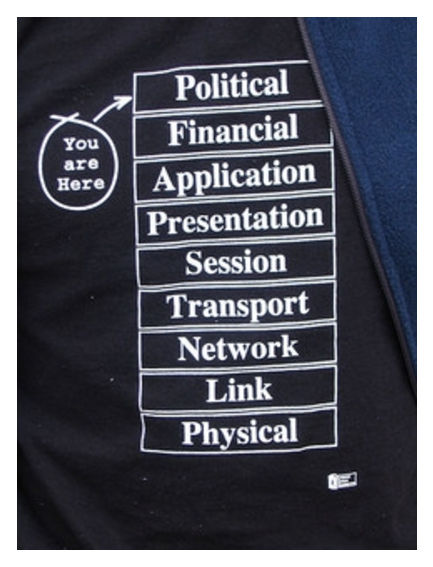
\includegraphics{ISO-9-layer-model-smaller.eps}
	\end{center}
\end{frame}

\begin{frame}
	\frametitle{Definitions}
	\begin{itemize}
		\item Certification
			\begin{itemize}
				\item Certification Test and Evaluation (CT\&E) phase
				\item Is performed by a \emph{certifier} or \emph{certification authority}.
			\end{itemize}
		\item Accreditation
			\begin{itemize}
				\item Security Test and Evaluation (ST\&E) phase
				\item Is performed by an \emph{accreditor} or Designated Approving Authority
					(DAA).
			\end{itemize}
		\item Re-certification event
		\item Accreditation Maintenance phase
	\end{itemize}
\end{frame}

\begin{frame}
	\frametitle{Methodology}
	\begin{itemize}
		\item I used a grounded theory methodology to discover what interesting things
			could be found in the data.
			\begin{itemize}
				\item This is especially suitable for software engineering investigations
					where controlled experiments are difficult and expensive to replicate.
			\end{itemize}
	\end{itemize}
\end{frame}

\begin{frame}
	\frametitle{Assumptions}
	\begin{itemize}
		\item Cross Domain Systems are always installed in an adversarial environment.
			\begin{itemize}
				\item Data owners do not trust one another.
				\item Accreditors represent data owners.
			\end{itemize}
		\item Accreditors have security clearance only to the necessary level.
			\begin{itemize}
				\item For example, some accreditors are cleared only for SECRET information
					and others have TOP SECRET security clearance.
			\end{itemize}
	\end{itemize}
\end{frame}

\begin{frame}
	\frametitle{Findings and New Results}
	\begin{enumerate}
		\item Model of inter-accreditor communication
			\begin{itemize}
				\item It satisfies the criteria of Spence and Akerlof for reliable signals
					in the presence of asymmetric information.
			\end{itemize}
		\item Method for predicting behaviour of accreditors
			\begin{itemize}
				\item Some undesirable information flows are forced.
				\item Some desirable information flows are inhibited.
				\item If Bell--LaPadula rules are followed, the security policy must be
					violated under some conditions.
			\end{itemize}
		\item Method for controlling the behaviour of certifiers
			\begin{itemize}
				\item The software developer of a CDS can exert some measure of control
					on the schedule of certification.
			\end{itemize}
	\end{enumerate}
\end{frame}

\begin{frame}
	\frametitle{Future Work}
	\begin{itemize}
		\item The presence of asymmetric information leads to arbitrage opportunities.
		\item Is there a market for risk?
		\item New tool: \emph{nihil obstat}
	\end{itemize}
\end{frame}

\begin{frame}
	\frametitle{Conclusion}
	\begin{itemize}
		\item The accreditor behaviour model is theoretically sound.
		\item It is possible to predict certain types of accreditor communication.
		\item The software developer has some control over the certification testing process.
	\end{itemize}
\end{frame}

\begin{frame}
	\frametitle{Merci}
	\begin{itemize}
		\item Thank you for inviting me here.
	\end{itemize}
\end{frame}

\end{document}

